\chapter{Design and Implementation}

\section{First Order Logic elements}

\begin{centering}
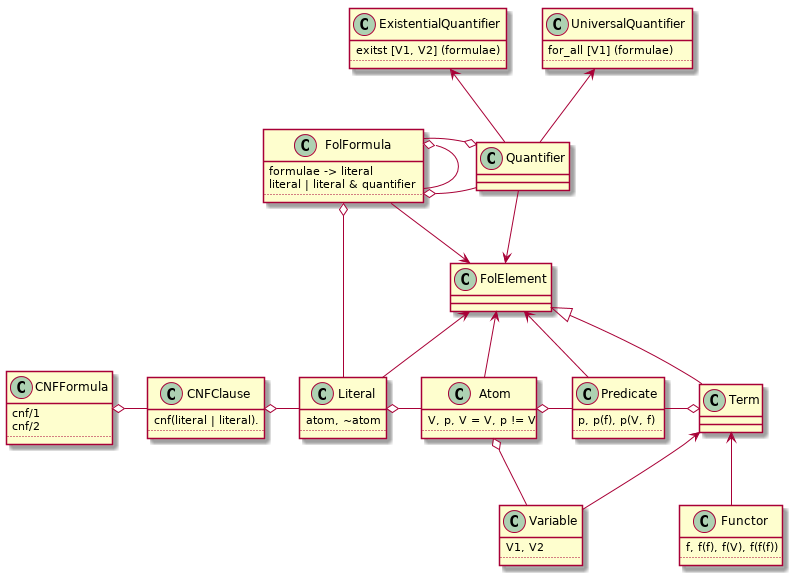
\includegraphics[width=\textwidth]{logic-formula-generator/fol/fol_elements.png}
\end{centering}

\section{CNF Generator parameters}

User defines generator in 3 steps.

\subsection{Allowed FOL elements}

In this step user defines set of allowed \gls{FOL} elements:
\begin{itemize}
	\item set of allowed functor arities $a_f = \{0, 1, 2,\dots\}$
	\item maximum recursion depth $n$ for functors
	\item set of allowed predicate arities $a_p = \{0, 1, 2,\dots\}$
	\item set of atom allowed connectives, that is no connective or/and any subset of $AllowedConnectives = \{=, !=\}$
	\item if negated literals are allowed
	\item set of allowed clause lengths $AllowedClausesLen = \{1,2,\dots\}$
	\item set of allowed number of clauses in formula $AllowedFormulaLen = \{1,2,\dots\}$
\end{itemize}

\subsection{Number of each element}
In this step iser defines what properties formula should have:
\begin{itemize}
	\item formula contains from $c_{min}$ to $c_{max}$ clauses, but the best solution is considered middle of this range
	\item formula contains from $l_{min}$ to $l_{max}$ literals, but the best solution is considered middle of this range
	\item TODO more params
\end{itemize}

\subsection{Names}
In this step user defines:
\begin{itemize}
	\item set of variable names $\{'v1','v2',\dots\}$
	\item set of functor names $\{'f1','f2',\dots\}$
	\item set of predicate names $\{'p1','p2',\dots\}$
\end{itemize}


\section{Basic algorithm}

The basic algorithm is greedy:
\begin{enumerate}
	\item Generate all possible formulas, based on user given values
	\item Pick first one that matches requirements
\end{enumerate}

Although presented algorithm is greedy, it can be optimized by solving equasions, that define user requirements.

\section{Optimizations}

CNF formula $F_{cnf}$ consists of clauses $c1, c2, \dots$. The order of clauses in not important.

\begin{align*}
	&F_{cnf}(x) = \{c1, c2, \dots\, cx\} \\
	\text{where }
		&x \text{ -- number of clauses in formula}
\end{align*}

If we group clauses by their length:
\begin{align*}
	&F_{cnf}(x) = \bigcup_{i=1}^c c_i \\
	\text{where }
		&c_i \text{ -- set of clauses with length i}
\end{align*}

Number of literals in formula can be represented as:
\begin{align*}
	l(x) &= x_1|c_1| + x_2|c_2| + \dots + x_x|c_x| = \sum_{i=1}^{x} x_i |c_i| \\
	x &= x_1 + x_2 + \dots + x_n \\
	c_i &\in AllowedClausesLen: \forall_{i \neq j} c_i \neq c_j  \\
	\text{where }
		&x \text{ -- number of clauses in formula} \\
		&l(x) \text{ -- number of literals in formula} \\
		&|c_i| \text{ -- number of clauses with length i} \\
\end{align*}

By solving above equation we can reduce greediness of algorithm. By using integer programming we can solve following equation within user defined thresholds and return random formula.

\begin{align*}
	l(x) &= \sum_{i=1}^{x} x_i |c_i| \\
	x &= \sum_i^x x_i \\
	l_{min} &< l(x) < l_{max} \\
	c_{min} &< x < c_{max} \\
	\text{where }
		&x \text{ -- number of clauses in formula} \\
		&l(x) \text{ -- number of literals in formula} \\
		&|c_i| \text{ -- number of clauses with length i} \\
\end{align*}

\section{Complexity}

\subsection{Number of functors}

Functor can contain variable or another functor.

How many types (ignore functor and variable names) of functors $f$ can be produced, knowing that
\begin{itemize}
	\item $n$ is recursion depth,
	\item $a$ is arity,
	\item subfunctors have arity less or equal to $a$?
\end{itemize}


\begin{align*}
	&f(n, a) =
	\begin{cases}
		a, \text{for } n = 0, \\
		a \sum_{i=n}^{i=1} \sum_{j=a}^{j=0} f(n-i,a-j) \\
	\end{cases} \\
\end{align*}

\subsection{Number of predicates}

Predicates can contain functors or variables.

How many types (ignoring predicate, functor and variable name) of predicates $P$ can be produced, knowing that:
\begin{itemize}
	\item functor arity $a_f$ is in range $[a_{f1}, a_{f2}]$,
	\item functor recursion depth $n$ is less or equal to $n_{max}$,
	\item $a_p$ is predicate arity?
\end{itemize}

\begin{align*}
	f_t(n_{max}, a_{fmin}, a_{fmax}) &= \sum_{i=0}^{n_{max}} \sum_{j=a_{f1}}^{a_{f2}} f(i, j), \\
	P(a_p) &=
	\begin{cases}
		1, \text{for } a_p = 0 \\
		(f_t(n_{max}, a_{fmin}, a_{fmax}) + 1)^{a_p}, \\
	\end{cases} \\
	\text{where} \\
	f_t(n_{max}, a_{fmin}, a_{fmax}) & \text{ -- total number of functors} \\
\end{align*}

\subsection{Number of atoms}

Atom can contain variabe or predicate. Atom connects items with binary mathematical connective: $=$ or $!=$.

How many types of atoms $A$ can be produced, knowing that:
\begin{itemize}
	\item predicate arity $a_p$ is given as set of $\{1,2,\dots\}$?
\end{itemize}

\begin{align*}
	A(a_p) &=
	\text{where} \\
	& \text{ -- total number of functors} \\
\end{align*}

\subsection{Number of literals}

\subsection{Number of clauses}

Clause $C$ can contain only literals. The order of literals is not important.

\begin{align*}
	&C = \{l1, 12, \dots\}
\end{align*}

How many different clauses can be produced, knowing that:
\begin{itemize}
	\item clause length is $x$
	\item given set of literals $L = \{l1, l2, \dots\}$, $\forall_{i,j \in L} i \neq j$
\end{itemize}

\begin{align*}
	&C(x) = \binom{|L|}{x}, \\
	\text{where }
	&|L| \text{ -- number of elements in L} \\
\end{align*}

\subsection{Number of cnf formulas}

How many different cnf formulas can be produced, knowing that:
\begin{itemize}
	\item formula contains $x$ clauses
	\item given set of clauses $C = \{c1, c2, \dots\}$, $\forall_{i,j \in L} i \neq j$
\end{itemize}

\begin{align*}
	&F_{cnf}(x) = \binom{|C|}{x}, \\
	\text{where }
	&|C| \text{ -- number of elements in C} \\
\end{align*}
